\documentclass{article}
\usepackage[utf8]{inputenc}
\usepackage{tikz}
\usepackage{amsmath}
\usepackage{ngerman}
\usepackage{ifthen}
\usepackage{ marvosym }
\usepackage[top=4cm,bottom=3cm,left=3cm,right=3cm]{geometry}
\usetikzlibrary{automata}
\newboolean{sol}
\newboolean{ex}

\newcommand{\menge}[2]{\ensuremath{\left\lbrace #1 \,\middle\vert\, #2 \right\rbrace}}
\newcommand{\harrypotter}{\Lightning}

%%%% Config here

% Show excercises
\setboolean{ex}{true}
% Show solutions
\setboolean{sol}{true}
%%%

\usepackage{float}
\newcommand{\aufgaben}[2]{
\ifthenelse{\boolean{ex}}{
\ifthenelse{\boolean{sol}}{
	\subsection{Aufgaben}
}{}}{}
\ifthenelse{\boolean{ex}}{#1}{}
\ifthenelse{\boolean{ex}}{
\ifthenelse{\boolean{sol}}{
	\subsection{Lösungen}
}{}}{}
\ifthenelse{\boolean{sol}}{#2}{}
}

\begin{document}
\ifthenelse{\boolean{ex}}{
	\ifthenelse{\boolean{sol}}{
		\title{Übungsaufgaben 2 mit Lösung}
	}{
		\title{Übungsaufgaben 2}
	}
}{
	\ifthenelse{\boolean{sol}}{
		\title{Lösungen 2}
	}{
		\title{Leeres Blatt 2}
	}
}
\author{Simon Stroh und Moritz von Looz \\ Fixes von Sebastian Ullrich, Joachim Priesner und Max Wagner}
\maketitle
\section{CH-2-Sprachen, CNF und CYK} 
\aufgaben{
\begin{enumerate}
\item Zeige unter Verwendung der Sprachen $\{a^mb^nc^n \mid  m,n > 0\}$ und $\{a^nb^nc^m \mid  m,n > 0\}$, dass die Menge die kontextfreien Sprachen nicht unter Schnittbildung abgeschlossen ist.
\item Zeige mit 1.\ und de Morgan, dass die kontextfreien Sprachen nicht unter Komplementbildung abgeschlossen sind.
\item Warum funktioniert folgender "`Beweis"' nicht?
\begin{quote}
Die Menge der kontextfreien Sprachen ist unter dem Kleene-Stern-Operator abgeschlossen. Für eine Grammatik $G$ mit Startsymbol $S$, welche die Sprache $A$ generiert, füge die Regel $S \rightarrow SS$ ein. Damit generiert $G'$ jetzt $A^*$.
\end{quote}
\item Gib eine Grammatik an, die die Sprache $L_1 = \menge{a^ib^jc^k}{ i = j\mbox{ oder }j = k}$ erzeugt.
\item Gib eine Grammatik in Chomsky-Normalform an, die die Sprache $L_2 = \{a^nb^n \mid  n \geq 1\}$ erzeugt, und verifiziere mit CYK, ob $aaaabbbb \in L_2$.
\item \begin{enumerate}
	\item Sei $C$ eine kontextfreie Sprache und $R$ eine reguläre Sprache. Zeige, dass die Sprache $C \cap R$ kontextfrei ist.
	\item Benutze a), um zu zeigen, dass die Sprache $A = \menge{w}{w \in \{a, b, c\}^\ast \text{ und } w \text{ enthält gleich viele a, b und c }}$ nicht kontextfrei ist.
\end{enumerate}
\end{enumerate}
}{
\begin{enumerate}
\item Beide Sprachen sind offensichtlich kontextfrei (eine Grammatik ist leicht anzugeben). Der Schnitt ist die bekanntermaßen nicht kontextfreie Grammatik $\{a^nb^nc^n\mid  n > 0\}$.
\item Seien $L_1$, $L_2$ kontextfrei. Angenommen, die kontextfreien Sprachen wären unter Komplementbildung abgeschlossen. Dann wäre $\overline{L_1} \cup \overline{L_2}$ und eben auch $\overline{\overline{L_1} \cup \overline{L_2}} = L_1 \cap L_2$ kontextfrei.
\item Der Beweis scheitert, weil das Startsymbol auf der rechten Seite von Regeln vorkommen kann. Betrachte etwa die Grammatik $G$ (für Sprache $A$) gegeben durch $S \rightarrow \# \mid  aSb$. Das nach Anleitung konstruierte $G'$ mit $S \rightarrow \# \mid  aSb \mid  SS$ kann das Wort $a\#\#b$ ableiten, welches nicht in $A^*$ liegt.
\item Konstruiere die Vereinigung wie in Aufgabe 1.1 für die Sprachen aus Aufgabe 1.2.
\item Die Grammatik sei durch die Produktionen gegeben:
\begin{align*}
S&\rightarrow AB\mid AX\\
X&\rightarrow SB\\
A&\rightarrow a \\
B&\rightarrow b \\
\end{align*}
\begin{figure}
\centering
	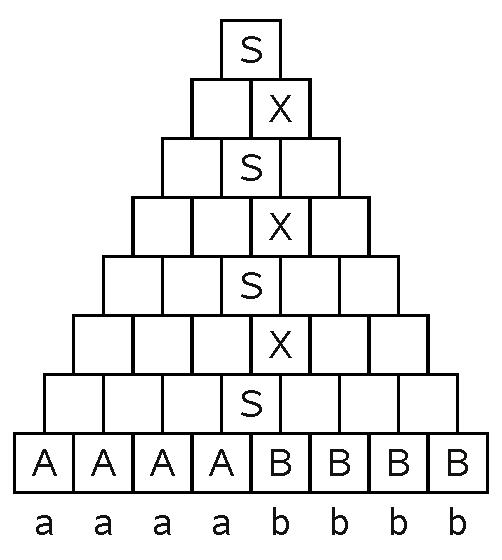
\includegraphics[scale=.5]{cyk.pdf}
\end{figure}
Das Wort ist in der Sprache:
\item \begin{enumerate}
	\item Sei $P$ der Kellerautomat, der $C$ durch akzeptierenden Endzustand erkennt, und $A$ der endliche Automat, der $R$ erkennt. Sei $Q$ die Zustandsmenge von $P$ und $Q'$ die Zustandsmenge von $A$. \\ Konstruiere einen Kellerautomaten $P'$, der $C \cap R$ erkennt, wie folgt: $P'$ hat die Zustandsmenge $Q \times Q'$. Er geht vor wie $P$, führt aber bei jedem Lesen eines Zeichens zusätzlich den entsprechenden Übergang aus $A$ aus. $P$ akzeptiert ein Wort $w$ genau dann, wenn er in einem Zustand aus $F_A \times F_P$ stoppt (wobei $F_A$ und $F_P$ die akzeptierenden Endzustände von $A$ und $P$ sind). Da $P'$ die Sprache $C \cap R$ erkennt, ist sie kontextfrei.
	\item Wenn $A$ kontextfrei wäre, dann wäre auch $A \cap R$ mit der regulären Sprache $R = a^*b^*c^*$ kontextfrei. Aber $A \cap R$ = $\menge{a^nb^nc^n}{n > 0}$ ist nicht kontextfrei \harrypotter.
\end{enumerate}
\end{enumerate}
}
\section{Ogdens und Pumping Lemma}
\aufgaben{
Sind folgende Sprachen kontextfrei?
\begin{enumerate}
\item $\{a^n\#a^{2n}\#a^{3n}\}$
\item $\menge{w\#t}{w\mbox{ ist Teilstring von }t \mbox{ und } w,t \in \{0,1\}^*}$
\item $\menge{w}{w \in \{a,b\} \mbox{und $w$ enthält doppelt soviele $a$ wie $b$ }}$
\item Das Komplement von $\{a^nb^n | n \geq 0\}$
\item $\menge{a\#b}{a,b \in \{0,1\}^* \mbox{ und } a \neq b}$
\end{enumerate}
}{
\begin{enumerate}
\item Widerlege mit Pumping Lemma.
\item Benutze Pumping Lemma für Wort $0^n1^n\#0^n1^n$.
\item Ja, konstruiere Grammatik.
\item Ja.
\item Ja (ohne Beweis).
\end{enumerate}
}
\section{Greibach-Normalform und Kellerautomaten}
\aufgaben{
\begin{enumerate}
    \item Konstruiere einen PDA für die folgende Grammatik:
\begin{align*}
S&\rightarrow asA \mid B \\
A&\rightarrow SS \mid a \\
B&\rightarrow bB \mid SA \\
\end{align*}

	\item Sei ein 2S-PDA definiert als Kellerautomat mit einem zusätzlichen zweiten Stack. In jedem Schritt wird ein Symbol oder Epsilon von der Eingabe gelesen, je eines von beiden Stacks gelesen und beliebig viele Symbole auf den ersten und den zweiten Stack geschrieben:
        $$\delta : Q \times ( \Sigma \cup \{\varepsilon\}) \times \Gamma^2 \rightarrow 2^{Q \times (\Gamma^*)^2}$$
        \begin{enumerate}
	\item Welche Klassen der Chomsky-Hierarchie erkennt ein 2S-PDA?
	\item Ist ein nichtdeterministischer 2S-PDA immer noch mächtiger als ein  deterministischer 2S-PDA?
\end{enumerate}	
\end{enumerate}
}{
\begin{enumerate}
    \item Der verfassende Tutor behauptet, dass die GNF aus 15 Produktionen besteht.
	\item Ein 2S-PDA ist äquivalent zu einer Turingmaschine: Das Lesen eines Symbols vom einen Stack und schreiben dieses Symbols auf den anderen Stack entspricht der Kopfbewegung einer Turingmaschine.
	\begin{enumerate}
		\item Genau die semientscheidbaren Sprachen, also CH-0.
		\item Nein, da NTMs genau dieselben Sprachen wie DTMs erkennen.
	\end{enumerate}
\end{enumerate}
}

\end{document}
